\documentclass{astroedu-lab}

\begin{document}

\pagestyle{plain}

\begin{problem}{\huge Сервер на основе esp32\\\\Измерение CO$_2$, температуры и влажности\\\\Выполнил Жданов Елисей Б01-205}

\section{Цель работы:}

Создать портативное устройство с возможностью выдачи показаний датчиков как на дисплей, так и на http сервер.

\section{Компоненты:}

1) Датчик SenseAir S8-0053

2) Датчик DHT 22(AM2302)

3) Дисплей IIC SSD1306

4) Контроллер ESP32-WROOM-32D

5) Аккумулятор 18650 с обвязкой питания

6) Провода, кнопки

7) Корпус, напечатанный на 3д принтере

\section{Оборудование:}

3д принтер, ПО для моделирования

Напильник, шуруповерт, инструменты постобработки

\section{Подключение}

Более подробно это описано в репозитории проекта

https://github.com/Elisey-e/Esp32-Multisensor-Server

\section{Включение}

\begin{figure}[!h]
	\centering
	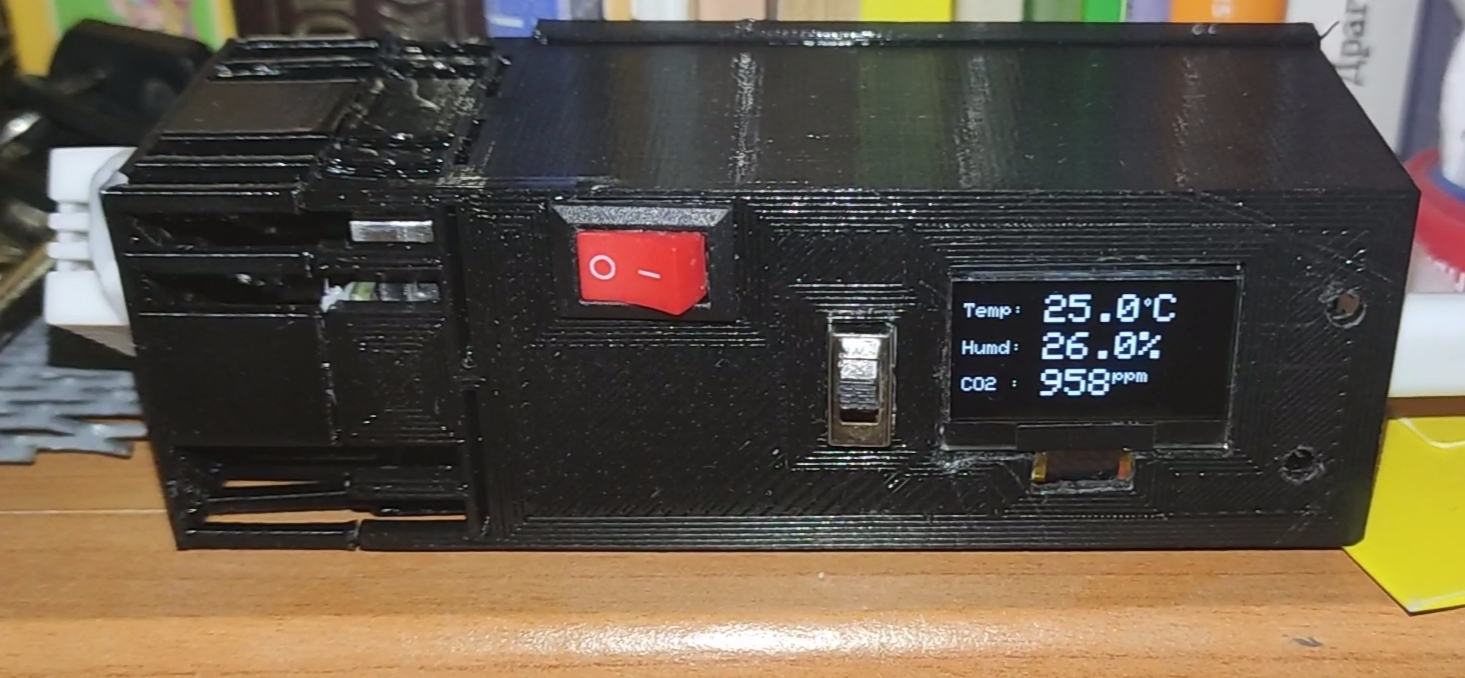
\includegraphics[width=0.9\textwidth]{release.jpg}
	\label{fig:boiler}
\end{figure}

Устройство запускается при подаче питания на плату esp либо по кабелю microusb, либо от аккумулятора 18650(красная кнопка). Также требуется активный сервер, указанный в программе при прошивке. При соблюдении условий устройство проходит инициализацию, на дисплее высвечиваются показания, а на сервере начинают обновляться данные

\begin{figure}[!h]
	\centering
	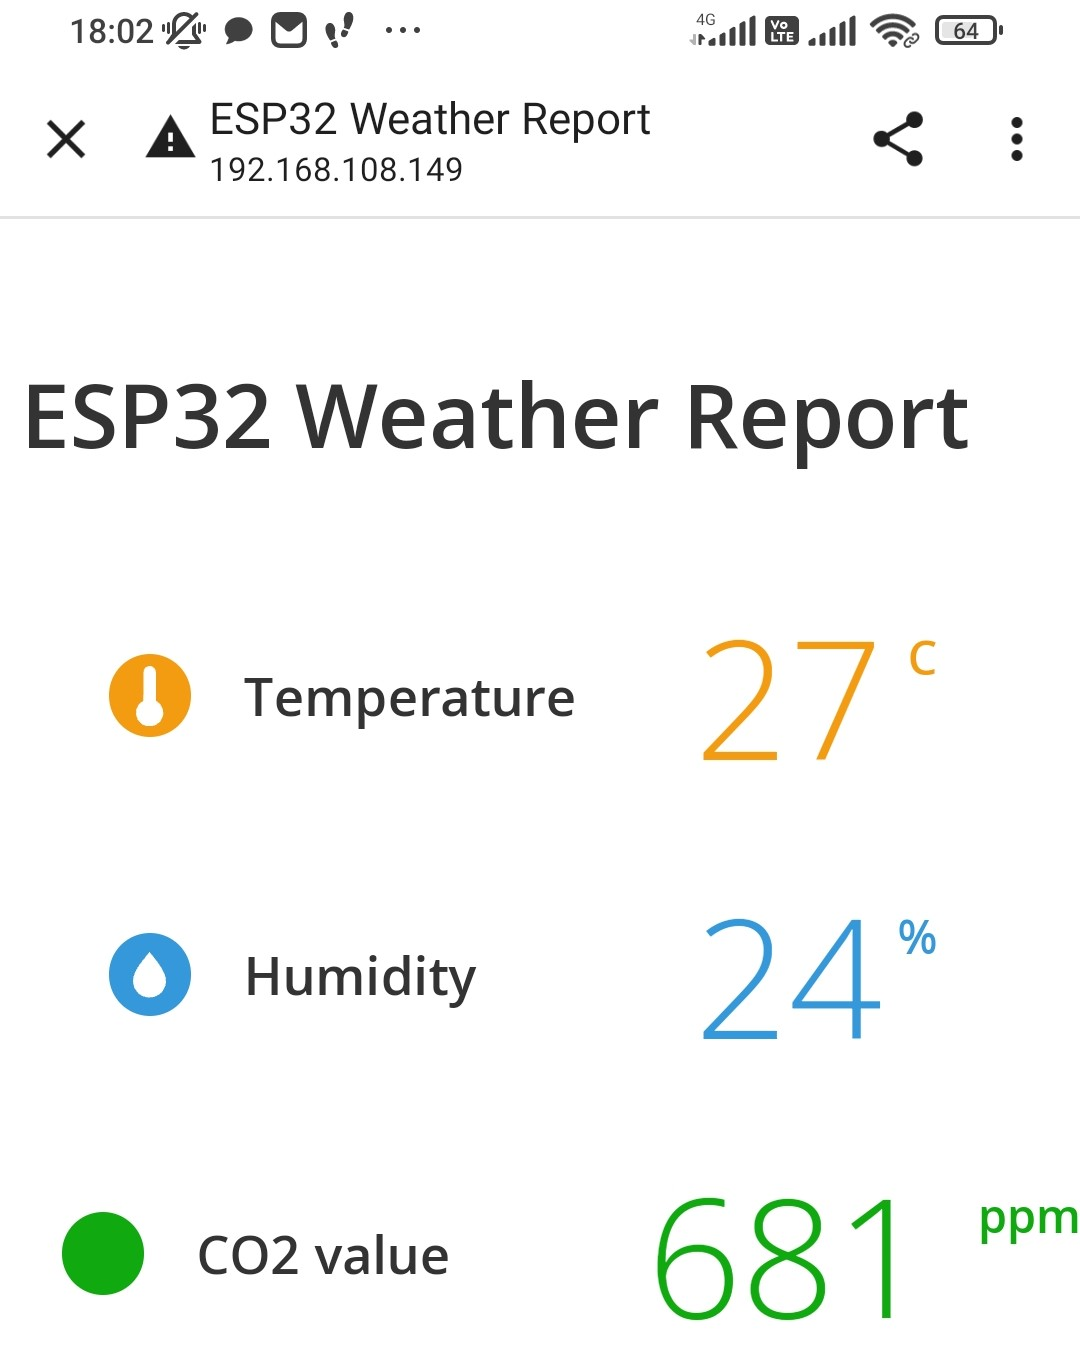
\includegraphics[width=0.5\textwidth]{ServerScreen.jpg}
	\label{fig:boiler}
\end{figure}

\section{Устройство}

Датчики подключены по распиновке, с использованием соответствущих свободных библиотек. Обновление веб страницы происходит с помощью AJAX, так, при подключении устройства к сети, страница сама начинает обновляться без перезагрузки. Специфические подробности прокомментированы в коде.

\section{Ресурсы}
$$
microkontroller.ru/esp32-projects/podklyuchenie-oled-displeya-k-modulyu-esp32/
$$
$$
raw.githubusercontent.com/KlausMu/esp32-co2monitor
$$
$$
blog.ifound.me/smarthome/podklyuchaem-k-esp8266-datchik-senseair-s8-0053/
$$
$$
github.com/KlausMu/esp32-co2monitor/tree/main?tab=readme-ov-file
$$

\end{problem}
\end{document}